\documentclass[12pt,titlepage,french]{article}
\usepackage{babel}
\usepackage{graphicx}
\usepackage[margin=2.5cm]{geometry}

\usepackage[hidelinks]{hyperref}
\usepackage{tabularx}
\usepackage[utf8]{inputenc}
\usepackage[T1]{fontenc}
\pagestyle{plain}

\usepackage{booktabs,makecell,tabu}
\usepackage{comment}
\renewcommand\theadfont{\bfseries}

\linespread{1.5}

\newcounter{firstbib}

\begin{document}
%\renewcommand{\thesection}{\arabic{section}} % utilisé pour spécifier la numérotation des sections

\begin{titlepage}
\newcommand{\HRule}{\rule{\linewidth}{0.5mm}}
\center

  
\includegraphics[width=0.45\textwidth]{../../ressources/img_logos/logo_polytech.png}\\[1cm]

  
\includegraphics[width=0.45\textwidth]{../../ressources/img_logos/logo_taglabs.png}


\HRule \\[0.4cm]
{ \huge \bfseries Rapport itération 3\\[0.15cm] }
Classification colorimétrique de nuages de points 3D\\
Version 1.0\\
Le \today \\
\HRule \\[1.5cm]
Ronan Collier,
Mathieu Letrone,
Tri-Thien Truong
\\[1cm]
\end{titlepage}

\tableofcontents % table des matières
\newpage
\listoffigures  % table des figures
\newpage

\section{Rappel des objectifs de l'itération}
Pour cette itération, nos objectifs étaient surtout concentrés sur l'amélioration de notre solution existante. En effet, nous avions réussi à créer un plugin sur le logiciel CloudCompare, en se basant sur le plugin existant "QPCL". Toutefois, nous voulions exporter notre projet sur un plugin à part, afin de rendre le code plus facile à maintenir, et de bien distinguer ce que nous développions, à ce qui était déjà présent.

Les tâches que nous nous sommes fixées sont les suivantes :

\begin{itemize}
  \item Refactoring du code / Exportation sur un nouveau Plugin
  \item Amélioration de la sélection de points dans le nuage
  \item Amélioration du filtrage RGB / Conversion LAB
  \item Intégration du Point picking, du filtrage multi-scans
\end{itemize}

\section{Production / réalisation durant l'itération}

Nous développerons ici chaque objectif que nous nous sommes fixé pour cette itération.

\subsection{Refactoring du code / Exportation sur un nouveau Plugin}

Nous avons pris le temps pour revoir notre structure du code, afin de l'exporter sur notre propre projet. Pour faire cela, nous nous sommes basé sur un template de plugin CloudCompare, disponible sur le git du projet. \newline

Ensuite, nous avons repris notre code développé sur le plugin QPCL, pour le mettre sur notre nouveau projet. Pour faire cela, nous avons dû enlever les dépendances avec QPCL (donc les méthodes de la bibliothèques PCL pour traiter des nuages de points). Nous avons donc utilisé uniquement les outils intégrés à CloudCompare, pour faire nos traitements. \newline

Nous aurions pu créer une dépendance avec le plugin QPCL et notre propre plugin, mais nous voulions d'abord voir s'il était possible de faire nos filtrages / segmentation avec les outils de CloudCompare, ce qui était effectivement le cas. Pour voir si notre choix était le bon, nous avons comparé notre ancienne méthode (utiliser la bibliothèque de PCL), et la nouvelle (uniquement CloudCompare). Le critère de comparaison a été au niveau du temps pour réaliser notre filtrage (RGB). \newline

Nous avons réalisé des tableaux comparatifs entre notre ancienne méthode d'implémentation (avec QPCL), et notre nouvelle implémentation (CloudCompare CC). \newline

\begin{figure}[!hbtp]
  \caption{\label{} Nuage de points de test}
  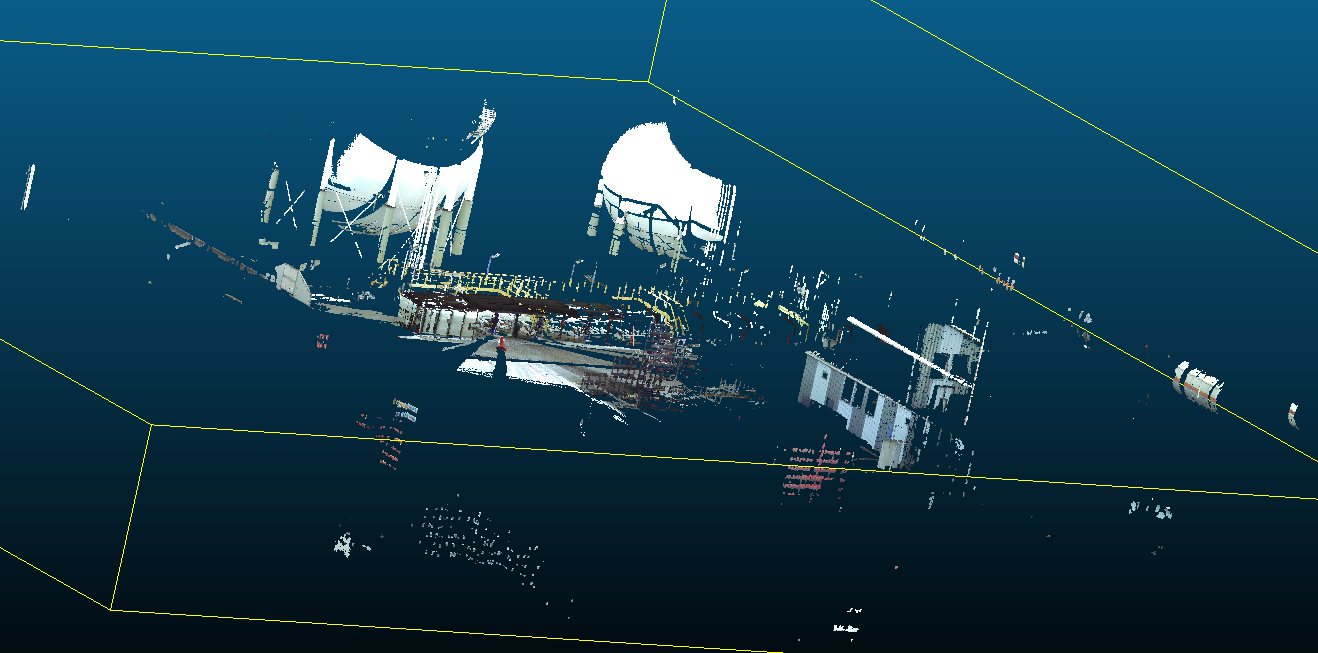
\includegraphics[width=1\textwidth]{./img/scan.png}
\end{figure}

Le fichier de test contient 22 649 423 points. Nous avons décidé de choisir un fichier très volumineux, puisque dans une situation réelle, tous les nuages de points seront aussi volumineux. Notre algorithme devra donc s'adapter à ce genre de jeu de données. De plus, les tests réalisés sur des nuages de points plus petits (de l'ordre de 100 x plus petit) apportaient des résultats très similaires, donc la comparaison n'était pas très représentative. \newline

\begin{figure}[!hbtp]
  \caption{\label{} Relevés des temps QPCL et CC}
  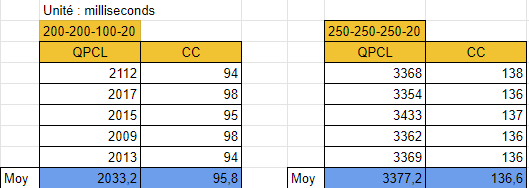
\includegraphics[width=1\textwidth]{./img/donnees.png}
\end{figure}

Nous pouvons voir dans la figure 2, les valeurs de temps, en millisecondes, relevées sur notre filtrage RGB du nuage de points de la figure 1. Le tableau de gauche permet de faire un filtrage sur les points de couleur jaunâtre (RGB : 200 - 200 - 100), avec une marge d'erreur de 20\%.

Pour comparer avec un filtrage où il y a un grand nombre de points à garder, nous avons fait un autre filtrage avec les points de couleur blanc (250 - 250 - 250, marge d'erreur de 20\%). \newline

Nous observons qu'il y a une grande différence entre les deux méthodes. Le filtrage avec des méthodes de CloudCompare uniquement, est beaucoup plus rapide qu'en utilisant QPCL. Notre deuxième méthode est de l'ordre d'environ 20 fois plus rapide que notre ancienne méthode. Nous avons donc un gain de temps énorme sur notre nouvelle méthode. \newline

Cela est probablement dû au fait qu'avant, nous utilisions une conversion du nuage de points d'un objet avec CloudCompare, en objet de PCL. Ensuite, nous réalisions le filtre avec ce type de nuage, pour ensuite reconvertir le nuage filtré en un objet CloudCompare, pour finalement l'afficher. Ces différentes étapes n'existent plus sur notre nouveau filtrage.

\subsection{Amélioration de la sélection de points dans le nuage}
Jusqu'à présent, la segmentation du nuage de point n'était qu'un simple filtrage des points par rapport à une valeur RGB de référence. Il s'agit d'une méthode répondant au besoin mais qui n'en demeure pas moins simpliste et manquant d'efficacité. \newline

Lors de nos recherches réalisées dans le cadre de la première itération, nous avons abouti à la découverte d'une nouvelle méthode de segmentation colorimétrique \cite{B01}. Cette 3ème itération devait permettre l'implémentation de ce nouvel algorithme. Cependant, les ajouts de nouvelles tâches ainsi que les imprévus nous ont freinés dans son implémentation. \newline

La segmentation est donc à l'heure actuelle dans un état embryonnaire. Seule la structuration de bases des méthodes est présente.

\subsection{Amélioration du filtrage RGB / Conversion LAB}

Suite aux retours de notre client, nous avons pu revoir l'utilisation du filtrage RGB implémenté lors de notre précédente itération. Une des propositions était d'utiliser qu'un seul point à choisir pour appliquer le filtrage RGB, et de la marge d'erreur pour établir les bornes des points à garder.

\begin{figure}[!hbtp]
  \caption{\label{} Ancienne interface et nouvelle interface filtrage RGB}
  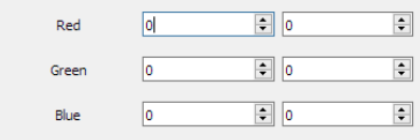
\includegraphics[width=0.4\textwidth]{./img/rgb_old.png}
\hspace*{1in}
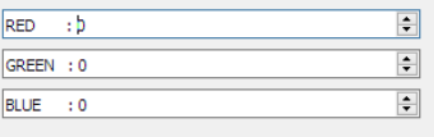
\includegraphics[width=0.4\textwidth]{./img/rgb_new.png}
\end{figure}

A gauche, nous pouvons observer l'ancienne interface (uniquement les champs pour le RGB), et à droite, la nouvelle interface. \newline

Suite à notre réunion de fin d'itération, l'idée de la sélection de deux points est plus intéressante au final, puisque cela nous permettra de sélectionner des bornes plus facilement. En effet, dans un nuage de points, un objet d'une certaine couleur peut avoir beaucoup de variation au niveau de cette couleur, selon l'endroit d'où il est pris par la station, la luminosité etc. \newline

La conséquence est donc le fait que les valeurs RGB des points peuvent énormément variées, malgré le fait que visuellement, nous avons la même couleur. En gardant la sélection de deux points, nous pourrons donc définir des bornes minimum et maximum des valeurs RGB, au lieu de faire varier la marge d'erreur, qui n'est pas forcément très pertinent sur notre problème.

En parallèle de la segmentation basée sur les valeurs RGB, le développement d'une autre basée sur l'espace colorimétrique CIElab. Cet espace permet de théoriquement de séparer la luminance de la chrominance ainsi cela pourrait résoudre les problèmes de luminosité imputés par les stations.
La conversion du RGB vers le LAB se fait en deux temps. D'abord, la conversion du RGB vers le XYZ (espace intermédiaire permettant le lien entre les deux) puis du XYZ vers le LAB. L'ensemble des calculs sont relativement simples, majoritairement des calculs matriciels.

Lors de la saisie des valeurs colorimétriques pour la segmentation, cette valeur sera convertie en LAB au même titre que l'ensemble des points du nuage.
La segmentation LAB est pour l'instant basée sur le même modèle que celle RGB, hormis qu'on ne teste que les composantes chromatiques des points (soit *a et *b).

Néanmoins, cette conversion a un coup d'exécution non négligeable par rapport à celle RGB .En effet, le temps d'exécution pour un même jeu de données sont en moyenne 30 fois plus long. Ce qui représente une augmentation non négligeable du temps total. D'autant, plus qu'à l'heure actuelle les résultats sont presque identiques. C'est pourquoi, il tâchera d'améliorer les algorithmes de la segmentation et déterminer si on doit encore travailler sur cet espace ou se concentrer sur le RGB.

\begin{figure}[!hbtp]
  \caption{\label{} Comparaison LAB et RGB en temps d'exécution}
  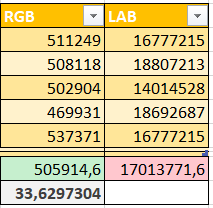
\includegraphics[width=0.4\textwidth]{./img/tableau_comparaisonRGB_LAB.png}
\end{figure}
\subsection{Intégration du Point picking, multi-scans}

Nous avons aussi dédié une partie de notre temps de cette itération, pour l'amélioration de l'utilisation de notre plugin sur le logiciel CloudCompare. En effet, le client a pu nous faire des retours sur l'utilisation directe de notre plugin.\newline

Les deux points les plus importants que nous voulions traiter sont le Point picking (le fait de pouvoir sélectionner un point directement sur le nuage de points, et récupérer les valeurs RGB), et le multi-scans. \newline

Le premier point était important par le fait que l'utilisateur final voudra une interface la plus simple et la plus pratique possible. Au lieu d'avoir l'obligation de taper manuellement les valeurs RGB (en passant donc par le point picking intégré au logiciel CloudCompare dans un premier temps), il aura la possibilité de cliquer sur le bouton qui activera la sélection d'un point sur le nuage. \newline

Le second point concernait plus l'utilisation du plugin par l'entreprise de façon générale, par rapport à leur fonctionnement. En effet, en situation réelle, l'entreprise possède plusieurs nuages de points d'un même lieu, avec des scans venant de stations positionnées à différents endroits. Le multi-scans permettra donc de faciliter le filtrage, puisque l'on veut dans la plupart des cas, filtrer tous les nuages du points correspondant à un lieu.

\begin{figure}[!hbtp]
  \caption{\label{} Nouvelle interface filtrage RGB}
  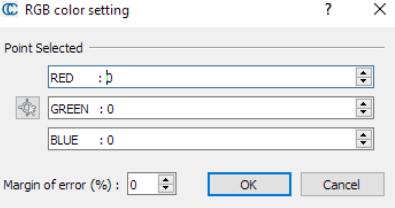
\includegraphics[width=0.65\textwidth]{./img/new_ui.png}
\end{figure}

Nous pouvons observer le point picking représenté par un bouton à gauche des champs RGB. Il est donc maintenant possible de saisir manuellement les valeurs, ou de cliquer sur le nouveau bouton, qui active le mode point picking de CloudCompare. L'utilisateur peut donc ensuite cliquer sur un point du nuage. Après son clic, s'il a bien cliqué sur un point, les champs RGB se remplissent automatiquement avec les valeurs RGB du point correspondant. Il peut toujours noter sa marge d'erreur, pour définir sa plage de points, et valider avec le bouton OK.

\section{Risques éliminés durant l'itération}
Durant cette itération, nous avons pu éliminer certains risques. En effet, le fait d'utiliser uniquement les outils de CloudCompare nous permet d'éviter d'être dépendant de la bibliothèque PCL. \newline

Bien sûr, il sera peut-être possible dans le futur, que nous aurions besoin d'utiliser cette bibliothèque pour certaines fonctions (par exemple, l'algorithme permettant de supprimer les points isolés). Mais pour l'instant, traiter les nuages de points avec le code que nous fournis CloudCompare nous suffit, et nous apporte un gain de temps non négligeable. \newline

Nous avions aussi des interrogations par rapport à notre méthode d'implémentation de notre plugin. En effet, le fait d'avoir notre propre plugin est une amélioration très importante quant à notre projet, puisque nous avons uniquement des fichiers qui servent au fonctionnement de notre plugin. L'implémentation est donc beaucoup plus aisée.

\section{Feedback}

Suite à notre présentation du sprint review, nous avons pu avoir des retours client. Tout d'abord, des retours sur l'interface utilisateur, bien qu'améliorée, elle reste perfectible. Le système de marge d'erreur est à revoir, il est en effet peu parlant pour un utilisateur et peu pertinent suivant les cas d'utilisations. Si les valeurs sont faibles, "la marge" en sera impactée et réduite. Au lieu, d'avoir cette marge, il serait mieux de choisir/sélectionner deux points dans le nuage, l'un serait la borne "basse" et l'autre la borne "haute". On choisirait ainsi, l'espace de couleur qu'on choisit de segmenter.

Ensuite, la possibilité de réaliser un premier process sur le nuage avant la segmentation, le process permettrai de discrétiser l'histogramme des couleurs, pour obtenir un effet cartoonesque. De ce fait, le problème des contrastes et différentes luminosités seraient déjà grandement palliés en plus de donner une meilleure idée des éléments gardés après la segmentation.

\section{Commentaires sur l'itération}

Cette section va présenter nos ressentis sur notre itération. Cela peut correspondre à comment nous avons pu gérer la charge de travail que nous avions prévu en début d'itération, des potentiels imprévus, points positifs/négatifs, et autres.

\subsection{Commentaires sur l'itération de façon générale}

Par rapport aux deux itérations précédentes, cette itération a été très rapide par rapport à ce que nous avions prévu. En effet, nous avons au maximum essayé de respecter nos délais définis dans le cahier des charges. Notre problème a été surtout par rapport au fait que nous avions eu une semaine de moins par rapport à notre réunion client/rendu de sprint review, ce qui nous a amené donc deux semaines de développement effectives (car la réunion de cette itération a été une semaine avant la fin de l'itération, nous devions donc être prêt pour la réunion, et non pour la fin d'itération). \newline

\subsection{Commentaires sur les méthodes de travail/changements de méthode}

Nous avons gardé les mêmes méthodes de travail, en essayant de se répartir les tâches les plus indivualisées possibles, pour éviter d'être dépendant du travail d'une autre personne. Le développement a été ici surtout freiné par le fait que c'est un travail surtout sur de la création d'algorithmes et de prise en main des technologies, ce qui requiert beaucoup de temps.

\section{Objectifs de la prochaine itération}

Durant cette itération, nous avons pu grandement mettre en ordre notre projet. Nous avons donc maintenant notre propre plugin. Il faut maintenant terminer ce qui était en cours, prendre en compte les retours du client, et continuer les tâches prévues du cahier des charges. Les tâches prévues sont donc les suivantes :

\begin{itemize}
  \item Intégration de fausses couleurs
  \item Revoir la marge d'erreur du filtrage RGB
  \item Terminer la nouvelle méthode de segmentation
  \item Toon mapping \newline
\end{itemize}

Pour la prochaine itération, il nous faudra prévoir la préparation pour notre deuxième soutenance, qui présentera nos premières solutions sur ce projet. Nous aurons une semaine de vacances, qui nous serviront justement à avancer sur le Ptrans.

\begin{figure}[!hbtp]
  \caption{\label{} Diagramme de Gantt détaillé - Sprint 4}
  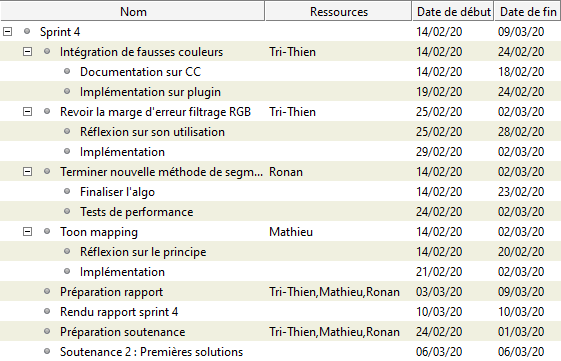
\includegraphics[width=1\textwidth]{./img/sprint_iteration_4_tableau.PNG}
  \raisebox{-1\height}
  {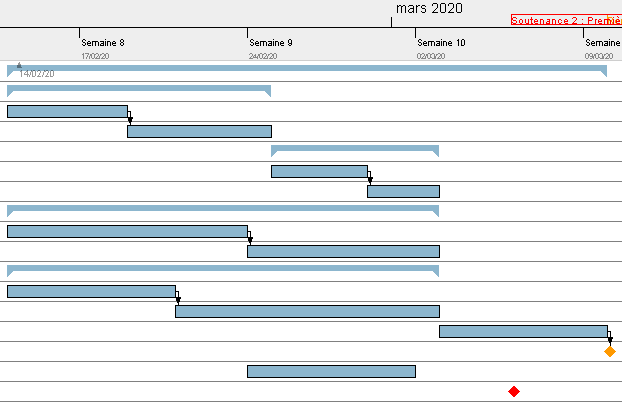
\includegraphics[width=1\textwidth]{./img/sprint_iteration_4_diagramme.PNG}} 
\end{figure}

\section{Résumé}
\subsection{Tâches principales réalisées dans l'itération}
\noindent\begin{tabu} to \textwidth {p{0.18\textwidth}X[c2]X[c]X[c4]}\toprule
  \thead{Tâche}&\thead{Responsable}&\thead{Statut}&\thead{Commentaire}\\\toprule
Refactoring du code / exportation sur un nouveau Plugin
& Ronan, Mathieu, Tri-Thien
& Achevé
& Fin de QPCL, plugin à part et indépendant.\\\midrule
Amélioration de la sélection de points dans le nuage
& Ronan
& En cours
& Continuer l'algo pour avoir une meilleure sélection des points.\\\midrule
Amélioration du filtrage RGB
& Tri-Thien
& Achevé
& Modification entre 2 points à 1 point \\\midrule
Conversion LAB
& Mathieu
& Achevé
& Comparaison de performances avec RGB\\\midrule
Point picking
& Tri-Thien
& Achevé
& Amélioration de l'interface pour cliquer sur un point, au lieu d'écrire manuellement les valeurs.\\\midrule
Multi-scans
& Ronan
& Achevé
& Sélection de plusieurs scans pour tous les filtrer en même temps.\\\bottomrule  \\
\end{tabu}

\subsection{Tâches principales à réaliser pour la prochaine itération}
\begin{itemize}
  \item Intégration de fausses couleurs
  \item Revoir la marge d'erreur du filtrage RGB
  \item Terminer la nouvelle méthode de segmentation
  \item Toon mapping
\end{itemize}
\begin{thebibliography}{3}

\bibitem{B01} Qingming Zhan, Yubin Liang, Yinghui Xiao, \textit{Color-based segmentation of point clouds}, 2009
\end{thebibliography}
\end{document}
